\section[\thesection \  Künstliche Neuronale Netze]{Künstliche Neuronale Netze}\label{sec:nn}

\begin{frame}{Neuronale Netze}

    \begin{itemize}
        \item was: NN lernt in gr Datenmenge Zusammenhänge und kann diese generalisieren so das es sie auch für neue daten anwenden kann
        \item wie: input daten mit zugehörigen outputs (hier gelabelte bilder) in Modell, dieses lernt iterativ die zusammenhänge
    \end{itemize}

    \vspace{1cm}

    \begin{center}
        \begin{columns}[T]
            \column{0.3\textwidth}
            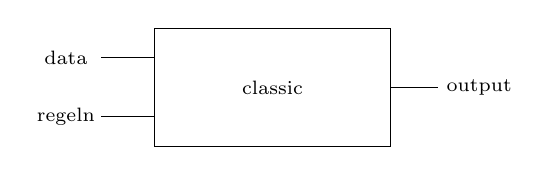
\begin{tikzpicture}[scale=0.75]
    \node at (0,1.5) {\scriptsize data};
    \node at (0,0.5) {\scriptsize regeln};
    \draw (0.6,1.5) -- (1.5,1.5);
    \draw (0.6,0.5) -- (1.5,0.5);
    \draw (1.5,0) rectangle (5.5,2);
    \node at (3.5,1) {\scriptsize classic};
    \draw (5.5, 1) -- (6.3, 1);
    \node at (7, 1) {\scriptsize output};
\end{tikzpicture}
            \column{0.3\textwidth}
            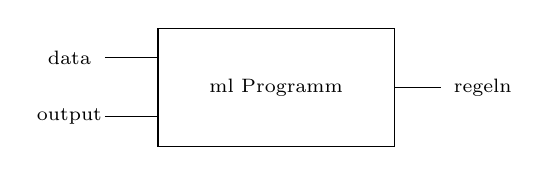
\begin{tikzpicture}[scale=0.75]
    \node at (0,1.5) {\scriptsize data};
    \node at (0,0.5) {\scriptsize output};
    \draw (0.6,1.5) -- (1.5,1.5);
    \draw (0.6,0.5) -- (1.5,0.5);
    \draw (1.5,0) rectangle (5.5,2);
    \node at (3.5,1) {\scriptsize ml Programm};
    \draw (5.5, 1) -- (6.3, 1);
    \node at (7, 1) {\scriptsize regeln};
\end{tikzpicture}
        \end{columns}
        
    \end{center}
    
\end{frame}
